\chapter{Формы}\label{chap:forms}
Я уже упоминал граничное условие: если данные приходят в приложение или
покидают его, мы должны их проверять. Вероятно, наиболее сложная проверка
происходит в формах.  Программировать формы не так просто; в идеальных
условиях мы хотели бы иметь решение, которое может следующее:

\begin{itemize}
    \item гарантировать, что данные корректны;

    \item преобразовывать строковые данные формы в типы данных Haskell;

    \item генерировать код HTML для отображения формы;

    \item генерировать Javascript, выполняющий валидацию на стороне клиента и
        предоставляющий более дружелюбные пользователю виджеты, например, для
        выбора даты;

    \item строить более сложные формы, объединяя вместе более простые;

    \item автоматически присваивать полям имена, которые гарантированно будут
        уникальными.
\end{itemize}

Пакет \footnotehref{http://hackage.haskell.org/package/yesod-form}{yesod-form}
предоставляет все эти возможности с помощью простого,
декларативного API. Он построен на базе виджетов Yesod для упрощения стилевого
оформления форм и применения Javascript надлежащим образом. И, как и везде в
Yesod, для обеспечения корректной работы используется система типов Haskell.

\section{Краткий обзор}
\includecode{08/synopsis.hs}

\section{Виды форм}
Погружение в непосредственное рассмотрение типов нам следует начать с обзора
различных видов форм. Их три категории:
\begin{description}
    \item[Аппликативные] \hfill \\
        Наиболее широко используемые (см. пример выше). Аппликативные формы
        позволяют нам объединять сообщения об ошибках друг с другом, сохраняя
        при этом декларативный высокоуровневый подход. Более детальную
        информацию об аппликативном подходе можно почерпнуть
        в~\footnotehref{http://www.haskell.org/haskellwiki/Applicative\_functor}%
        {Haskell-вики}.

    \item[Монадические] \hfill \\
        Более мощная альтернатива аппликативным. Гибкость достигается за счёт
        несколько большей многословности. Бывают полезны, если необходимо
        создать форму, которая не укладывается в стандартный двухстолбцовый
        формат.

    \item[Формы для ввода] \hfill \\
        Используются только для получения ввода. Не генерируют никакого HTML для
        получения ввода пользователя. Полезны для взаимодействия с уже
        существующими формами.
\end{description}

Кроме того существует ряд различных переменных для каждого вида формы и поля,
которые вам захочется установить:
\begin{itemize}
    \item Обязательное поле или нет?
    \item Данные должны передаваться методом GET или POST?
    \item Есть у поля значение по умолчанию или нет?
\end{itemize}

Главная цель~--- минимизировать число определений полей и позволить им
работать в максимально возможном количестве контекстов. Одним из результатов
этого явилось то, что мы пришли к добавлению нескольких дополнительных параметров для
каждого поля. В обзоре вы, наверное, заметили слово \lstinline'areq' или
дополнительный параметр \lstinline'Nothing'. В рамках данной главы мы обсудим
зачем они нужны, а пока примите себе, что сделав эти параметры явными, мы
получили возможность повторно использовать отдельные поля
(например,~\lstinline'intField') большим количеством различных способов.

Краткое замечание по поводу именования. Каждая форма имеет однобуквенный
префикс (\texttt{A}, \texttt{M} или~\texttt{I}), который используется в
нескольких местах, как например в \lstinline'MForm'. Мы также будем
использовать~\lstinline'req' и~\lstinline'opt' для обозначения обязательных
(required) и необязательных (optional) полей соответственно. В итоге,
обязательное аппликативное поле мы создаём с помощью~\lstinline'areq', а
необязательное поле для ввода данных~--- с помощью~\lstinline'iopt'.

\section{Типы}
Модуль \texttt{Yesod.Form.Types} определяет несколько типов. Мы не будем
описывать все доступные типы, а сконцентрируемся на основных. Давайте начнём с
простых:
\begin{description}
    \item[Enctype] \hfill \\
        Тип кодировки: либо \lstinline'UrlEncoded', либо \lstinline'Multipart'.
        Этот тип данных объявляет экземпляр для класса
        типов~\lstinline'ToHtml', так что вы можете его использовать
        непосредственно в шаблонах Hamlet.

    \item[FormResult] \hfill \\
        Имеет одно из трёх возможных состояний: \lstinline'FormMissing'~---
        если данные не были переданы, \lstinline'FormFailure'~--- если
        произошла ошибка при разборе формы (например, не заполнено обязательное
        поле или содержимое поля некорректно) или~\lstinline'FormSuccess',
        когда всё прошло гладко.

    \item[FormMessage] \hfill \\
        Представляет все различные сообщения, которые могут быть сгенерированы,
        в виде типа данных. Например, \lstinline'MsgInvalidInteger'
        используется библиотекой для указания, что предоставленное текстовое
        значение не является целым числом. Хранение этих данных хорошо
        структурированным образом, даёт вам возможность предоставить любую
        желаемую функцию рендеринга для интернационализации вашего приложения.
\end{description}

Также есть типы данных, используемые для определения отдельных полей. Мы
определяем поле как отдельную порцию информации, например, число, строка или
адрес электронной почты. Поля собирают вместе для построения форм.

\begin{description}
    \item[Field] \hfill \\
        Определяет два вида функциональности: как преобразовать текстовый ввод
        пользователя в значение языка Haskell и как создавать виджет, который
        будет показан пользователю. \texttt{yesod-form} определяет набор
        отдельных полей в модуле \lstinline'Yesod.Form.Fields'.

    \item[FieldSettings] \hfill \\
        Основная информация о том, как поле следует отображать: отображаемое
        имя, необязательная подсказка, и, возможно, явно заданные атрибуты
        \lstinline'id' и~\lstinline'name'. (Если ничего не указано, то они
        генерируются автоматически.) Обратите внимание, что
        \lstinline'FieldSettings' предоставляет экземпляр~\lstinline'IsString',
        так что, когда вам понадобится указать значение
        типа~\lstinline'FieldSettings', вы можете обойтись просто строковым
        литералом. Как мы и сделали во введении.
\end{description}

И, наконец, мы добрались до важного: до самих форм. Есть три типа данных для
форм: \lstinline'MForm' для монадических, \lstinline'AForm' для аппликативных и
\lstinline'FormInput' для форм ввода данных. \lstinline'MForm' на самом деле
является синонимом типа для стека монад, который предоставляет следующие
возможности:
\begin{itemize}
    \item Монада \lstinline'Reader' предоставляет нам параметры, отправленные
        пользователем, основной тип данных и список языков, которые
        поддерживаются пользователем. Последние два используются для рендеринга
        сообщений из \lstinline'FormMessage' для поддержки интернационализации
        (подробнее об этом ниже).

    \item Монада \lstinline'Writer' отслеживает \lstinline'Enctype'. Для формы
        значение всегда будет~\lstinline'UrlEncoded', за исключением случая,
        когда присутствует поле для загрузки файла. Тогда будет использовано
        значение~\lstinline'Multipart'.

    \item Монада \lstinline'State' хранит созданные имена и идентификаторы для
        полей.
\end{itemize}

Форма \lstinline'AForm' устроена похожим образом. Однако, есть несколько важных различий:
\begin{itemize}
    \item Она генерирует список значений типа~\lstinline'FieldView',
        используемые для отслеживания, что будет показано пользователю. Это
        позволяет нам оперировать абстракцией отображения форм, выбирая
        соответствующую функцию для отрисовки её на странице в самом конце. Во
        введении мы использовали \lstinline'renderDivs', которая создаёт связку
        тегов div. Два других варианта: \lstinline'renderBootstrap'
        и~\lstinline'renderTable'.

    \item У неё нет экземпляра \lstinline'Monad'. Задача
        \lstinline'Applicative' заключается в том, чтобы позволить форме
        выполниться целиком, собрать как можно больше информации, и выдать
        конечный результат. Это не работает в контексте \lstinline'Monad'.
\end{itemize}

\lstinline'FormInput' ещё проще: она возвращает либо список ошибок, либо результат.

\section{Преобразование}
<<Минуточку>>,~--- скажете вы. <<Вы говорите, что во введении использовались
аппликативные формы, но я уверен, что сигнатура типа
указывает~\lstinline'MForm'. Не были ли они монадическими?>>. Да, верно,
итоговая форма, которую мы создали, была монадической. Но на самом деле
произошло вот что: мы преобразовали аппликативную форму в монадическую.

Повторюсь, наша цель заключается в том, чтобы повторно использовать как можно
больше кода и минимизировать число функций в API. А монадические формы
являются более мощными, чем аппликативные, поэтому, грубо говоря, всё, что
может быть выражено аппликативными формами, может быть выражено и
монадическими. Есть две основные функции, которые нас здесь выручают:
\lstinline'aformToForm' преобразует любую аппликативную форму в монадическую,
а \lstinline'formToAForm' преобразует определённые виды монадических форм в их
аппликативные варианты.

<<\textbf{Ещё} минутку>>,~--- настаиваете вы. <<Я не видел никаких
\lstinline'aformToForm'!>>. Это тоже верно.  Функция~\lstinline'renderDivs'
позаботилась об этом для нас.

\section{Создание аппликативных форм}
Теперь, когда я (надеюсь) убедил вас, что во введении мы действительно имели
дело с аппликативными формами, давайте попытаемся понять, как они создаются.
Начнём с простого примера:

\begin{lstlisting}
data Car = Car
    { carModel :: Text
    , carYear  :: Int
    }
  deriving Show

carAForm :: AForm Handler Car
carAForm = Car
    <$> areq textField "Model" Nothing
    <*> areq intField  "Year" Nothing

carForm :: Html -> MForm Handler (FormResult Car, Widget)
carForm = renderTable carAForm
\end{lstlisting}%$

Здесь мы явным образом разделили аппликативные и монадические формы.
В~\lstinline'carAForm' мы использовали операторы~\lstinline'<$>'
и~\lstinline'<*>'. Это не должно удивлять; они почти всегда используются в
коде, использующем аппликативный стиль. Также у нас по одной строчке для каждой
записи нашего типа данных~\lstinline'Car'. Вероятно, также не удивляет, что мы
использовали \lstinline'textField' для записи с типом~\lstinline'Text' и
\lstinline'intField' для записи с типом~\lstinline'Int'.

Давайте взглянем поближе на функцию~\lstinline'areq'. Её (упрощённая)
сигнатура типа~--- \lstinline'Field a -> FieldSettings -> Maybe a -> AForm a'.
Первый аргумент определяет тип данных поля, как его разбирать и как
отображать.  Следующий аргумент, \lstinline'FieldSettings', даёт нам метку,
подсказку, имя и идентификатор поля. В данном случае, мы используем выше
упомянутый экземпляр~\lstinline'IsString' для~\lstinline'FieldSettings'.

А что с \lstinline'Maybe a'? Этот аргумент даёт нам необязательное
значение по умолчанию.  Например, если мы хотим, чтобы наша форма подставляла
для года машины значение по умолчанию <<2007>>, мы будем использовать
\lstinline'areq intField "Year" (Just 2007)'. Мы даже можем подняться на
уровень выше, и получить форму, которая принимает необязательный аргумент,
задающий значения по умолчанию.

\begin{lstlisting}
carAForm :: Maybe Car -> AForm Handler Car
carAForm mcar = Car
    <$> areq textField "Model" (carModel <$> mcar)
    <*> areq intField  "Year"  (carYear  <$> mcar)
\end{lstlisting}%$

\subsection{Необязательные поля}
Предположим, что нам нужно необязательное поле (например, цвет машины). Всё
что нужно~--- это воспользоваться функцией \lstinline'aopt'.

\begin{lstlisting}
carAForm :: AForm Handler Car
carAForm = Car
    <$> areq textField "Model" Nothing
    <*> areq intField  "Year"  Nothing
    <*> aopt textField "Color" Nothing
\end{lstlisting}%$

Как и в случае обязательных полей, последний аргумент~--- необязательное
значение по умолчанию.  В итоге, тут получается двойное оборачивание
в~\lstinline'Maybe'. Это может показаться чрезмерным, но существенно упрощает
написание кода, который принимает в качестве необязательного параметра форму со
значениями по умолчанию, как в следующем примере.

\begin{lstlisting}
carAForm :: Maybe Car -> AForm Handler Car
carAForm mcar = Car
    <$> areq textField "Model" (carModel <$> mcar)
    <*> areq intField  "Year"  (carYear  <$> mcar)
    <*> aopt textField "Color" (carColor <$> mcar)

carForm :: Html -> MForm Handler (FormResult Car, Widget)
carForm = renderTable $ carAForm $ Just $ Car "Forte" 2010 $ Just "gray"
\end{lstlisting}

\section{Валидация}
Как мы можем сделать, чтобы наша форма принимала только машины, созданные после
1990 года?  Если вы помните, мы говорили выше, что \lstinline'Field' сам по
себе содержит информацию о том, что представляет собой корректное значение. То
есть, всё что нам надо сделать~--- это написать новый \lstinline'Field', верно?
Это будет несколько утомительно. Вместо этого, давайте изменим уже существующее
поле.

\begin{lstlisting}
carAForm :: Maybe Car -> AForm Handler Car
carAForm mcar = Car
    <$> areq textField    "Model" (carModel <$> mcar)
    <*> areq carYearField "Year"  (carYear  <$> mcar)
    <*> aopt textField    "Color" (carColor <$> mcar)
  where
    errorMessage :: Text
    errorMessage = "Ваша машина чересчур стара, купите новую!"

    carYearField = check validateYear intField

    validateYear y
        | y < 1990 = Left errorMessage
        | otherwise = Right y
\end{lstlisting}

Хитрость в функции~\lstinline'check'. Она принимает функцию
(\lstinline'validateYear'), которая возвращает либо сообщение об ошибке, либо
модифицированное значение поля. В этом примере, мы вообще не изменяли значение.
Это самый частый случай использования. И так как этот вид проверки довольно
распространён, у нас есть сокращение:

\begin{lstlisting}
carYearField = checkBool (>= 1990) errorMessage intField
\end{lstlisting}

Функция \lstinline'checkBool' принимает два параметра: условие, которое должно
быть выполнено, и сообщение об ошибке, которое следует отобразить в случае
невыполнения.

\begin{remark}
Вы могли заметить явное указание \lstinline'Text' в сигнатуре типа функции
\lstinline'errorMessage'. При использовании расширения OverloadedStrings это
необходимо. Чтобы поддерживать интернационализацию, сообщения могут иметь
множество различных типов, и у GHC нет возможности определить, какой
экземпляр~\lstinline'IsString' вам нужен.
\end{remark}

Это замечательно~--- гарантировать, что наша машина не очень старая. А если мы
хотим убедиться в том, что указанный год не из будущего? Чтобы получить текущий
год, нам потребуется выполнить действие ввода/вывода. Для таких случаев нам
потребуется функция~\lstinline'checkM', которая позволяет нашему проверочному
коду выполнять произвольные действия:

\begin{lstlisting}
    carYearField = checkM inPast $ checkBool (>= 1990) errorMessage intField

    inPast y = do
        thisYear <- liftIO getCurrentYear
        return $ if y <= thisYear
            then Right y
            else Left ("У Вас есть машина времени!" :: Text)

getCurrentYear :: IO Int
getCurrentYear = do
    now <- getCurrentTime
    let today = utctDay now
    let (year, _, _) = toGregorian today
    return $ fromInteger year
\end{lstlisting}%$

Функция \lstinline'inPast' вернёт результат типа \lstinline'Either' в
монаде~\lstinline'Handler'. Мы используем \lstinline'liftIO getCurrentYear',
чтобы получить текущий год, и затем сравниваем его с годом, указанным
пользователем. Также обратите внимание, как мы можем связывать вместе несколько
валидаторов.

\begin{remark}
Так как валидатор \lstinline'checkM' работает в монаде \lstinline'Handler', он
имеет доступ ко всем операциям, которые вы можете обычно выполнять в Yesod.
Это особенно полезно для выполнения операций с базой данных, которые мы
рассмотрим в главе~\nameref{chap:persistent}.
\end{remark}

\section{Поля посложнее}
Наше поле для ввода цвета хорошее, но не совсем дружественное пользователю.
Что мы хотим на самом деле~--- это выпадающий список.

\begin{lstlisting}
data Car = Car
    { carModel :: Text
    , carYear :: Int
    , carColor :: Maybe Color
    }
  deriving Show

data Color = Red | Blue | Gray | Black
    deriving (Show, Eq, Enum, Bounded)

carAForm :: Maybe Car -> AForm Handler Car
carAForm mcar = Car
    <$> areq textField "Model" (carModel <$> mcar)
    <*> areq carYearField "Year" (carYear <$> mcar)
    <*> aopt (selectFieldList colors) "Color" (carColor <$> mcar)
  where
    colors :: [(Text, Color)]
    colors = [("Red", Red), ("Blue", Blue), ("Gray", Gray), ("Black", Black)]
\end{lstlisting}%$

Функция \lstinline'selectFieldList' принимает список пар. Первый элемент
пары~--- это текст, который отобразится пользователю в выпадающем списке, а
вторым элементом является соответствующее значение Haskell. Конечно, код выше
выглядит повторяющимся; мы можем получить тот же результат воспользовавшись
экземплярами \lstinline'Enum' и \lstinline'Bounded', которые GHC автоматически
выводит для нас.

\begin{lstlisting}
colors = map (pack . show &&& id) $ [minBound..maxBound]
\end{lstlisting}%$

Интервал \lstinline'[minBound..maxBound]' даёт нам список всех отличных друг от
друга значений типа~\lstinline'Color'. Мы затем применяем~\lstinline'map'
и~\lstinline'&&&' (так называемый <<оператор разветвления>> (fan-out operator)),
превращая его в список пар.

Некоторые люди предпочитают выпадающим спискам переключатели.  К счастью, это
изменение в одно слово.

\begin{lstlisting}
carAForm = Car
    <$> areq textField               "Model" Nothing
    <*> areq intField                "Year"  Nothing
    <*> aopt (radioFieldList colors) "Color" Nothing
\end{lstlisting}%$

\section{Выполнение форм}
В какой-то момент у нас возникнет необходимость воспользоваться нашими
прекрасными формами и получить некоторые результаты.  Для этого в нашем
распоряжении есть целый ряд различных функций, каждая из которых имеет своё
назначение. Я пройдусь по всем, начиная с самых распространённых.

\begin{description}
    \item[runFormPost] \hfill \\
        Функция выполнит вашу форму с любыми предоставленными POST параметрами.
        Если запрос не является POST--запросом, вернёт \lstinline'FormMissing'.
        Функция автоматически вставляет маркер безопасности (security token) в
        виде скрытого поля для предупреждения
        кросс-сайтовых~(\footnotehref{http://en.wikipedia.org/wiki/Cross-site\_request\_forgery}%
        {CSRF}) атак.

    \item[runFormGet] \hfill \\
        Аналог \lstinline'runFormPost' для GET-параметров. Чтобы отличить
        обычную загрузку страницы через GET от отправки GET формы, включает в
        форму дополнительное скрытое поле~\lstinline'_hasdata'. И, в отличие
        от~\lstinline'runFormPost', не содержит защиты от кросс-сайтовых атак.

    \item[runFormPostNoToken] \hfill \\
        То же что и \lstinline'runFormPost', но не включает (или не требует)
        маркера безопасности CSRF.

    \item[generateFormPost] \hfill \\
        Вместо привязки к существующим POST параметрам, действует так, будто
        их нет. Может быть полезна, когда вам нужно сгенерировать новую форму
        после того, как предыдущая была отправлена, например, в мастере форм.

    \item[generateFormGet] \hfill \\
        То же что и \lstinline'generateFormPost', но для GET.
\end{description}

Тип возвращаемого значения первых трёх функций~---
\lstinline'((FormResult a, Widget), Enctype)'.  \lstinline'Widget' уже будет
включать любые ошибки валидации и ранее отправленные значения.

\section{Интернационализация}
В этой главе уже было несколько ссылок на интернационализацию. Эта тема
подробнее освещена в своей собственной~\hyperref[chap:i18n]{главе}, но, так как
она имеет глубокое влияние на \lstinline'yesod-form', я хотел дать краткий обзор.
Идея поддержки интернационализации в Yesod состоит в том, чтобы иметь
типы данных для представления сообщений. Каждый сайт может иметь
экземпляр~\lstinline'RenderMessage' для конкретного типа данных, который будет
переводить сообщение в соответствии со списком языков, принимаемых клиентом.
Как результат, есть несколько моментов, о которых вам следует знать:
\begin{itemize}
    \item  Для каждого сайта автоматически создаётся
        экземпляр~\lstinline'RenderMessage' для типа~\lstinline'Text', так что
        вы можете просто использовать простые строки, если не заботитесь о
        поддержке интернационализации. Однако, вам изредка может потребоваться
        использовать явные сигнатуры типов.

    \item Все сообщения в \lstinline'yesod-form' выражаются в терминах типа
        данных~\lstinline'FormMessage'.  Поэтому, для использования \lstinline'yesod-form'
        вам нужен соответствующий экземпляр~\lstinline'RenderMessage'. Простая
        реализация, которая использует английский вариант перевода по
        умолчанию, будет выглядеть так:
\begin{lstlisting}
instance RenderMessage App FormMessage where
    renderMessage _ _ = defaultFormMessage
\end{lstlisting}
        Такой экземпляр автоматически предоставляется каркасом сайта.
\end{itemize}

\section{Монадические формы}
Зачастую, простая вёрстка форм достаточна, и тут аппликативные формы
превосходны. Иногда, однако, вы захотите получить более настраиваемый вид вашей
формы.
\begin{figure}[tbph]
  \centering
  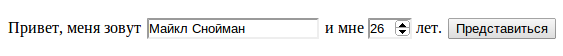
\includegraphics[width=\textwidth]{08-forms-image-01.png}
  \caption{Нестандартная вёрстка формы}
\end{figure}

В таких случаях следует использовать монадические формы. Они несколько более
многословны, чем их аппликативные родственники, но эта многословность
позволяет вам получить полный контроль над тем, как форма будет выглядеть.
Чтобы получить такую же форму, как приведённая выше, мы могли бы написать
что-то подобное следующему:
\includecode{08/monadic-forms.hs}

Подобно аппликативной функции~\lstinline'areq' мы используем \lstinline'mreq'
для монадических форм.  (И, конечно, есть \lstinline'mopt' для необязательных
полей).  Но здесь есть существенное различие: \lstinline'mreq' возвращает нам
пару значений.  Вместо скрытия значения типа~\lstinline'FieldView' и
автоматической его вставки в виджет, мы получаем управление вставкой по своему
усмотрению.

Тип данных \lstinline'FieldView' содержит ряд записей с информацией о поле
формы. Самая важная из них~--- \lstinline'fvInput', которая и есть фактическое
поле формы. В этом примере мы также использовали~\lstinline'fvId', которая
возвращает нам HTML атрибут~\texttt{id} тега~\texttt{input}. В нашем примере
мы её использовали, чтобы задать ширину поля.

Вас, наверное, интересует, что это за значения <<Это не используется>> и <<И это
тоже>>.  Функция~\lstinline'mreq' принимает вторым аргументом значение
типа~\lstinline'FieldSettings'.  Так как для \lstinline'FieldSettings'
существует экземпляр \lstinline'IsString', такие строки по сути раскрываются
компилятором в:

\begin{lstlisting}
fromString "Это не используется" == FieldSettings
    { fsLabel = "Это не используется"
    , fsTooltip = Nothing
    , fsId = Nothing
    , fsName = Nothing
    , fsClass = []
    }
\end{lstlisting}

В случае аппликативных форм, значения~\lstinline'fsLabel'
и~\lstinline'fsTooltip' использовались при построении HTML. В случае же
монадических форм, Yesod не генерирует для нас никаких HTML-обёрток, и поэтому
эти значения игнорируются. Однако, мы храним параметр
типа~\lstinline'FieldSettings', чтобы позволить вам при желании переопределять
атрибуты~\texttt{id} и~\texttt{name} ваших полей.

Ещё один интересный момент~--- значение~\lstinline'extra'. Формы типа GET
добавляют поле для обозначения отправки, а POST формы добавляют признак
безопасности для предупреждения кросс-сайтовых атак.  Если вы не включите это
дополнительное скрытое поле, то отправка форм закончится неудачей.

Всё остальное довольно-таки тривиально. Мы создаём наше
значение~\lstinline'personRes' из значений~\lstinline'nameRes'
и~\lstinline'ageRes', а затем возвращаем кортеж, включающий полученное значение
типа~\lstinline'Person' и виджет для формы. А в функции~\lstinline'getHomeR'
всё также, как для аппликативной формы. В действительности, вы могли бы
заменить монадическую форму на аппликативную, и код всё равно работал бы.

\section{Формы ввода данных}
Аппликативные и монадические формы выполняют как генерацию HTML, так и разбор
данных.  Иногда вам нужно только последнее, например, когда где-то уже создана
форма, или если вы хотите генерировать форму динамически, используя
Javascript. В этих случаях вам пригодятся формы ввода данных.

Они аналогичны аппликативным и монадическим с некоторыми различиями:
\begin{itemize}
    \item Вы используете \lstinline'runInputPost' и \lstinline'runInputGet'.

    \item Вы используете \lstinline'ireq' и \lstinline'iopt'. Эти функции
        теперь принимают только 2 аргумента: тип рассматриваемого поля и его
        имя (т.е. значение HTML атрибута~\texttt{name}).

    \item После выполнения формы, она возвращает значение. Она не возвращает
        виджет или тип кодировки.

    \item В случае ошибок проверки данных, возвращается страница с сообщением
        об ошибке <<некорректные аргументы (invalid arguments)>>.
\end{itemize}

Вы можете переписать предыдущий пример с помощью форм ввода данных. Однако,
стоит заметить, что эта версия менее дружественна пользователю. Если вы
допустите ошибку при заполнении аппликативной или монадической формы, то вы
вернётесь на ту же страницу с ранее введёнными данными, а сообщение об ошибке
укажет, что надо исправить. При использовании форм ввода данных пользователь
получит просто сообщение об ошибке.

\includecode{08/input-forms.hs}

\section{Пользовательские поля}
Поля, которые встроены в Yesod, скорее всего покроют большую часть ваших
потребностей для работы с формами. Но иногда вам может понадобиться что-то
более специализированное.  К счастью, вы можете создавать новые поля в Yesod
самостоятельно. Конструктор~\lstinline'Field' принимает три значения:
\lstinline'fieldParse' принимает список значений, отправленных пользователем,
и возвращает один из трёх результатов:
\begin{itemize}
    \item Сообщение об ошибке в случае, если проверка данных закончилась
        неудачей.

    \item Разобранное значение.

    \item \lstinline'Nothing', указывающее на то, что данные не были
        предоставлены.
\end{itemize}

Последний случай может несколько удивить. Может показать, что Yesod может
автоматически понять, что информации не было предоставлено, если входной список
пуст. Но на самом деле, для некоторых типов полей отсутствие любых входных
данных является, фактически, корректным значением. Флажки, например, сообщают о
сброшенном состоянии, посылая пустой список.

И почему список? Не лучше ли \lstinline'Maybe'? Не всегда. В случае группы
флажков или списков с возможностью множественного выбора у вас будет множество
виджетов с одним и тем же именем. Мы используем этот трюк в нашем примере ниже.

Вторая значение в конструкторе~--- это \lstinline'fieldView', которое формирует
виджет для отображения пользователю. У этой функции такие аргументы:
\begin{itemize}
    \item Атрибут~\texttt{id}.

    \item Атрибут~\texttt{name}.

    \item Другие произвольные атрибуты.

    \item Результат в виде значения типа~\lstinline'Either'. Будет содержать либо
        необработанный ввод (если обработка не удалась), либо успешно
        обработанное значение. Поле \lstinline'intField'~--- великолепный
        пример того, как это работает. Если вы введёте \textrm{42}, результатом
        будет~\lstinline'Right 42'. Но если вы введёте \textrm{черепаха}, то
        результат будет~\lstinline'Left "черепаха"'. Это позволит вам заполнить
        атрибут~\texttt{value} вашего тега~\texttt{input} для организации
        последовательного пользовательского интерфейса.

    \item значение типа~\lstinline'Bool' для обозначения, является ли поле
        обязательным.
\end{itemize}

Последний аргумент конструктора~--- значение \lstinline'fieldEnctype'. Если вы
имеете дело с загрузкой файлов, должно быть равно~\lstinline'Multipart', в
противном случае~--- \lstinline'UrlEncoded'.

В качестве маленького примера мы создадим новый тип поля~--- поле для
подтверждения пароля. В нём будет два элемента для ввода текста (оба с одним и
тем же значением атрибута~\texttt{name}), и оно будет возвращать сообщение об
ошибке, если пароли не совпадают. Заметьте, что в отличие от большинства
полей, новое поле \emph{не} предоставляет атрибуты~\texttt{value} для
тегов~\texttt{input}, потому что вы \textbf{никогда} не захотите отправлять
обратно введённый пользователем пароль в свой HTML.

\begin{lstlisting}
passwordConfirmField :: Field Handler Text
passwordConfirmField = Field
    { fieldParse = \rawVals _fileVals ->
        case rawVals of
            [a, b]
                | a == b -> return $ Right $ Just a
                | otherwise -> return $ Left "Пароли не совпадают"
            [] -> return $ Right Nothing
            _ -> return $ Left "Вы должны ввести оба значения"
    , fieldView = \idAttr nameAttr otherAttrs eResult isReq ->
        [whamlet|
            <input id=#{idAttr} name=#{nameAttr} *{otherAttrs} type=password>
            <div>Подтверждение:
            <input id=#{idAttr}-confirm name=#{nameAttr} *{otherAttrs} type=password>
        |]
    , fieldEnctype = UrlEncoded
    }

getHomeR :: Handler Html
getHomeR = do
    ((res, widget), enctype) <- runFormGet $ renderDivs
        $ areq passwordConfirmField "Пароль" Nothing
    defaultLayout
        [whamlet|
            <p>Результат: #{show res}
            <form enctype=#{enctype}>
                ^{widget}
                <input type=submit value="Сменить пароль">
        |]
\end{lstlisting}

\section{Значения, приходящие не от пользователя}
Представьте себе, что вы пишите приложение для размещения блогов и хотите
сделать форму для ввода пользователями сообщения в блог. Сообщение блога будет
содержать четыре элемента:
\begin{itemize}
    \item Заголовок.
    \item Содержимое в виде HTML.
    \item Идентификатор автора.
    \item Дата публикации.
\end{itemize}

Мы хотим, чтобы пользователь вводил только первые два значения. Идентификатор
пользователя должен определяться автоматически по результатам аутентификации
пользователя (эту тему мы ещё не рассматривали), а для даты публикации должно
использоваться текущее время. Вопрос, как нам сохранить простой аппликативный
синтаксис и в то же время получить значения, которые не вводятся пользователем?

Ответ: используя две вспомогательные функции:
\begin{itemize}
    \item \lstinline'pure' позволяет завернуть простое значение в значение
        аппликативной формы.

    \item \lstinline'lift' позволяет выполнить произвольное действие
        монады~\lstinline'Handler' внутри аппликативной формы.
\end{itemize}

Давайте посмотрим на пример использования этих функций:
\includecode{08/nonuser-values.hs}

\section{Выводы}
Формы в Yesod делятся на три вида. Аппликативные используются чаще всего, так
как предоставляют красивый интерфейс и простой для использования API.
Монадические формы дают больше возможностей, но их сложнее использовать. Формы
ввода данных полезны, когда вам надо просто принять данные пользователя, не
генерируя сложных виджетов.

Из коробки Yesod предоставляет несколько различных типов полей для форм. Для их
использования вам необходимо указать вид формы и является ли поле обязательным
или нет. Для этого есть шесть вспомогательных функций: \lstinline'areq',
\lstinline'aopt', \lstinline'mreq', \lstinline'mopt', \lstinline'ireq'
и~\lstinline'iopt'.

Формы обладают большой мощью. Они могут автоматически вставлять код на
Javascript, чтобы облегчить вам получение более привлекательных элементов
управления, как, например, диалог выбора даты из библиотеки jQuery UI. Формы
также полностью готовы для включения интернационализации, так что вы можете
поддерживать глобальное сообщество пользователей. А в случае более
специфических потребностей, вы можете привязать функции валидации данных для
существующих полей, или реализовать своё поле <<с чистого листа>>.
